\documentclass{article}

% if you need to pass options to natbib, use, e.g.:
%     \PassOptionsToPackage{numbers, compress}{natbib}
% before loading neurips_2021

% ready for submission
\usepackage[preprint]{neurips_2021}


% to compile a preprint version, e.g., for submission to arXiv, add add the
% [preprint] option:
%     \usepackage[preprint]{neurips_2021}

% to compile a camera-ready version, add the [final] option, e.g.:
%     \usepackage[final]{neurips_2021}

% to avoid loading the natbib package, add option nonatbib:
%    \usepackage[nonatbib]{neurips_2021}

\usepackage[utf8]{inputenc} % allow utf-8 input
\usepackage[T1]{fontenc}    % use 8-bit T1 fonts
\usepackage[colorlinks=true]{hyperref}       % hyperlinks
\usepackage{url}            % simple URL typesetting
\usepackage{booktabs}       % professional-quality tables
\usepackage{amsfonts}       % blackboard math symbols
\usepackage{nicefrac}       % compact symbols for 1/2, etc.
\usepackage{microtype}      % microtypography
\usepackage{xcolor}         % colors
\usepackage{graphicx}       % graphics
\usepackage{lipsum}


\title{Predicting Excess Mortality during the Covid 19 Pandemic via Demographic Features}

% The \author macro works with any number of authors. There are two commands
% used to separate the names and addresses of multiple authors: \And and \AND.
%
% Using \And between authors leaves it to LaTeX to determine where to break the
% lines. Using \AND forces a line break at that point. So, if LaTeX puts 3 of 4
% authors names on the first line, and the last on the second line, try using
% \AND instead of \And before the third author name.

\author{%
  Joschka Strüber\\
  Matrikelnummer 5980381\\
  \texttt{joschka.strueber@student.uni-tuebingen.de}
}

\begin{document}

\maketitle

\begin{abstract}
  We are planning to use the collection of \href{https://github.com/owid/covid-19-data}{Covid 19 data from Our World in Data} to test the statistical significance of excess mortality since the emergence of Covid compared to previous years. Furthermore, we want to use linear regression to examine the influence of demographic and structural variables on mortality rates with a particular focus on vaccination rates.
\end{abstract}

\section{Introduction}

\lipsum[1]

\section{Excess mortality during the COVID-19 pandemic}

\lipsum[2]
\lipsum[3]

\begin{figure}[t]
	\centering
	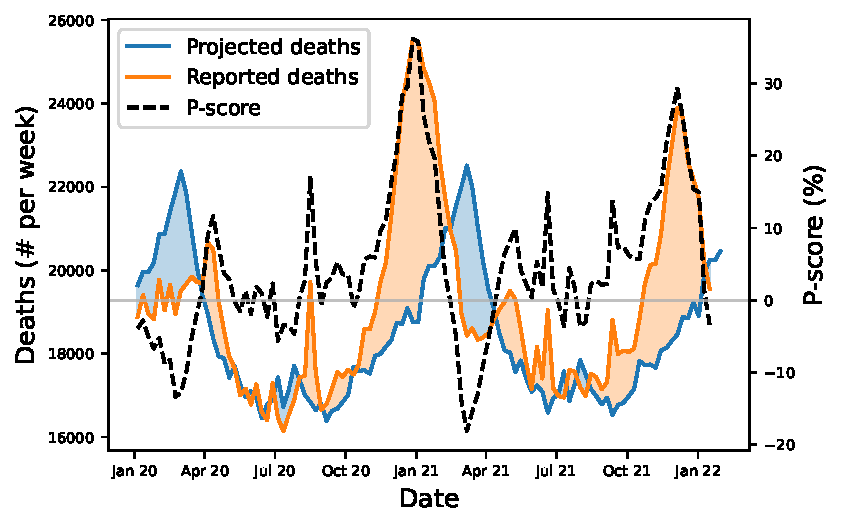
\includegraphics[width=0.8\linewidth]{fig/fig_em_intro}
	\caption[Blub]{text}
\end{figure}

\lipsum[2]

\lipsum[3]

\section{Demography as predictor of excess mortality}

\lipsum[1]

\begin{figure}[t]
	\begin{minipage}{0.3\linewidth}
		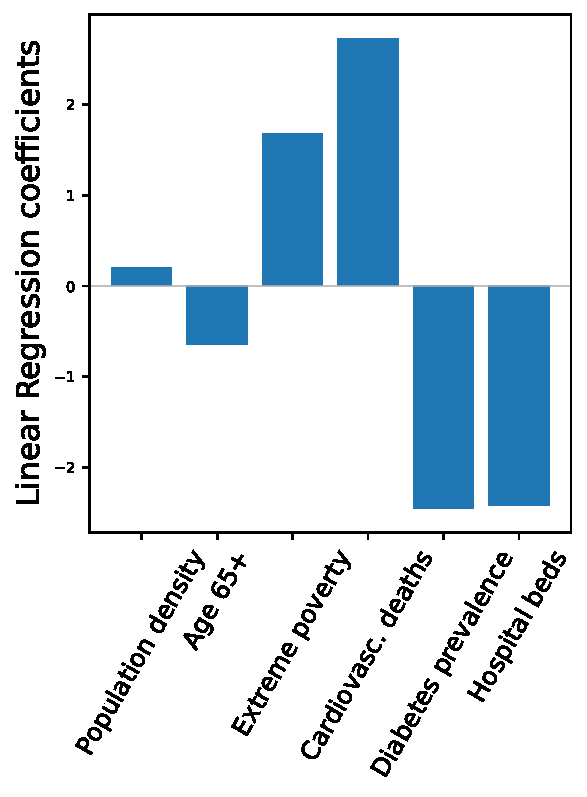
\includegraphics[width=\linewidth]{fig/fig_linear_regression_em}
	\end{minipage}\hfill
	\begin{minipage}{0.65\linewidth}
		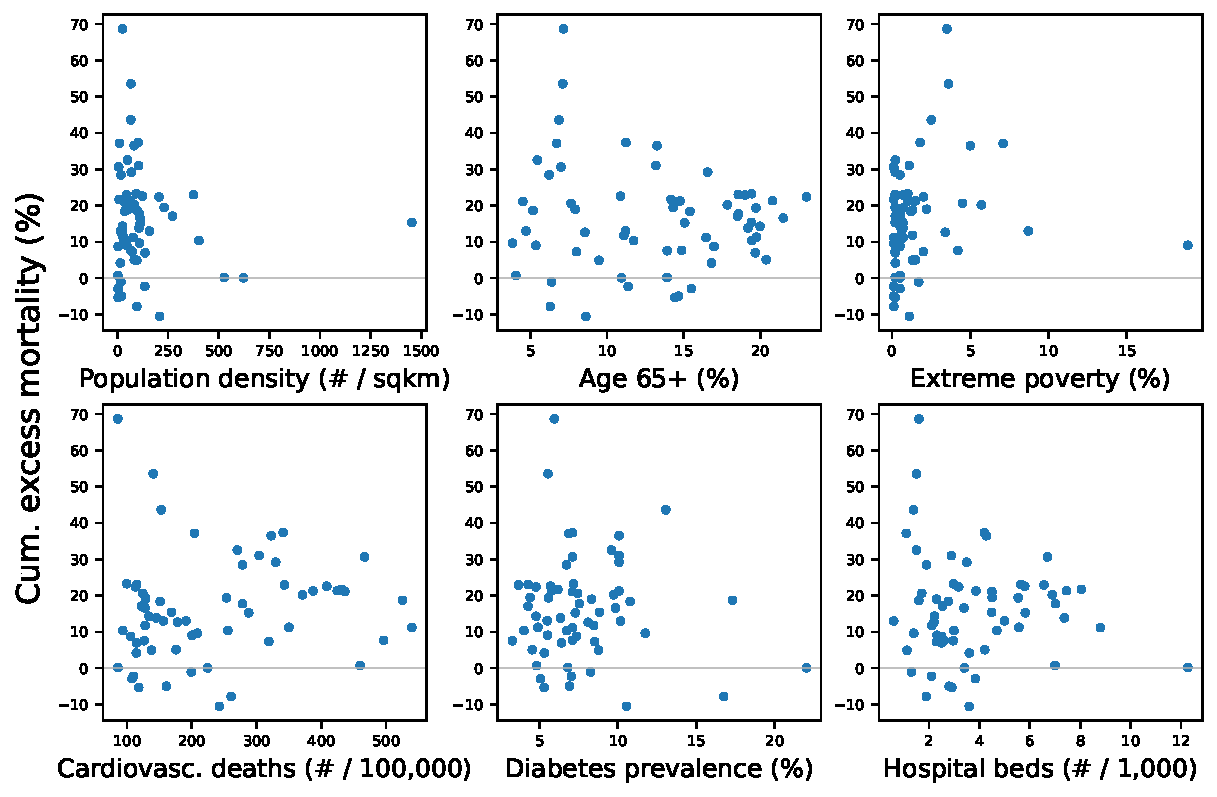
\includegraphics[width=\linewidth]{fig/fig_em_correlation}
	\end{minipage}
\end{figure}

\lipsum[1]

\section{The effect of vaccinations}

\lipsum[1]

\section{Conclusion}

\lipsum[1]

\end{document}
